\input{./_path-to-root.ltx}
\documentclass[\PathToRoot/\ProjectName]{subfiles}
\whenstandalone{\externaldocument{\PathToRoot/\ProjectName}}

\begin{document}

\begin{figure}[htb] 
  \centering
  \caption{Wealth distribution robustness: risk aversion sensitivity}
  \whenintegrated{\label{fig:LorenzPts_robustness_CRRA}} 
  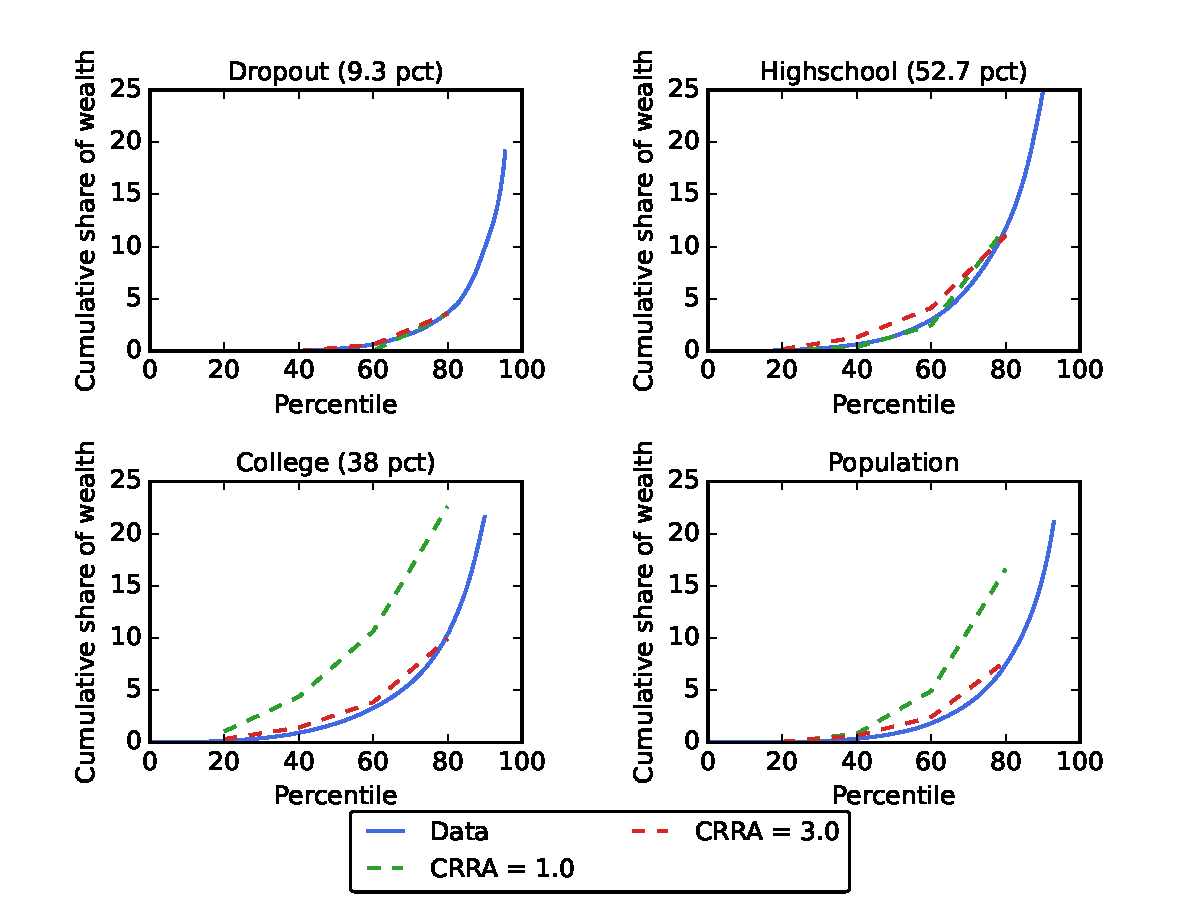
\includegraphics[width=.9\textwidth]{\PathToRoot/images/LorenzPoints_robustness_CRRA}

  \medskip
  \noindent\parbox{\textwidth}{\footnotesize
    \textbf{Note}: This figure tests robustness of wealth distribution fit to risk aversion specification
    (Appendix~\ref{sec:robustness}).
    The model maintains excellent fit to empirical wealth distributions across education groups
    when varying the coefficient of relative risk aversion ($\gamma$) from 1.0 to 3.0.
    The precautionary saving motive adapts through discount factor re-estimation while preserving
    the model's core empirical performance, demonstrating structural robustness of the estimation
    methodology for different preference specifications commonly used in macroeconomic analysis.
  }
\end{figure}

\vspace{0.5em}

% Smart bibliography: Only include bibliography if standalone AND has citations
\smartbib

\end{document}
